%!TEX root = Report.tex
\chapter{Einführung}\label{sec:introduction}

Im Gebiet der Hochtemperatur Solar-Chemie (z.B. für die Herstellung von Syngas durch den Zn/ZnO-Zyklus) sind zuverlässige Temperaturmessungen der Fluide von zentraler Bedeutung. Da die Wärmestrahlung proportional zur vierten Potenz der Temperatur ist, fällt diese bei höheren Temperaturen (ab $800^\circ$C) ins Gewicht und übernimmt eine viel wichtigere Rolle. Das Thermoelement, das für die Messung der Gastemperatur zuständig ist, beginnt deswegen bei höheren Temperaturen zu lügen, weil es nicht nur vom heissen Fluid sondern auch von der Strahlung des heissen Reaktors geheizt wird. In der Abbildung \ref{fig:reactor} sieht man ein solches Solar-Reaktor im Betrieb.\\


\begin{figure}[H]
\centering
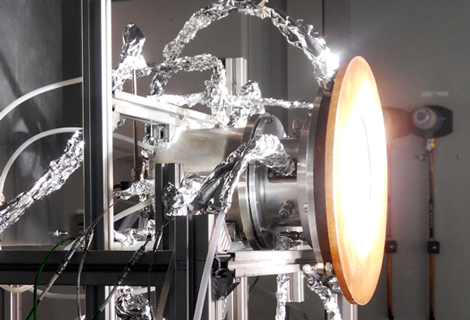
\includegraphics[width=0.5\textwidth]{pics/solar_reactor.png}
\caption{Reaktor im Betrieb. Quelle: \cite{caltech}}
\label{fig:reactor}
\end{figure}

Den oben erwähnten Effekt kann man verringen indem man das Thermoelement mit einem Strahlungsschild umschliesst um den Strahlungsaustausch mit der Umgebung zu verkleinern. Durch den schnellen Fluss des Betriebsgases, wird das Thermoelement durch Konvektion annähernd auf die eigentliche Gastemperatur abgekühlt. Die bekannte erzwungene Konvektion hilft uns dann die Messabweichung am Thermoelement zu beschreiben und zu quantifizieren. Wie dieses Effekt praktisch realisiert wird, wird im nächsten Kapitel im Detail erklärt. 